\documentclass[tikz,border=4mm]{standalone}
\usepackage[T1]{fontenc}
\usepackage{lmodern}
\usetikzlibrary{arrows.meta,positioning,calc}
\begin{document}
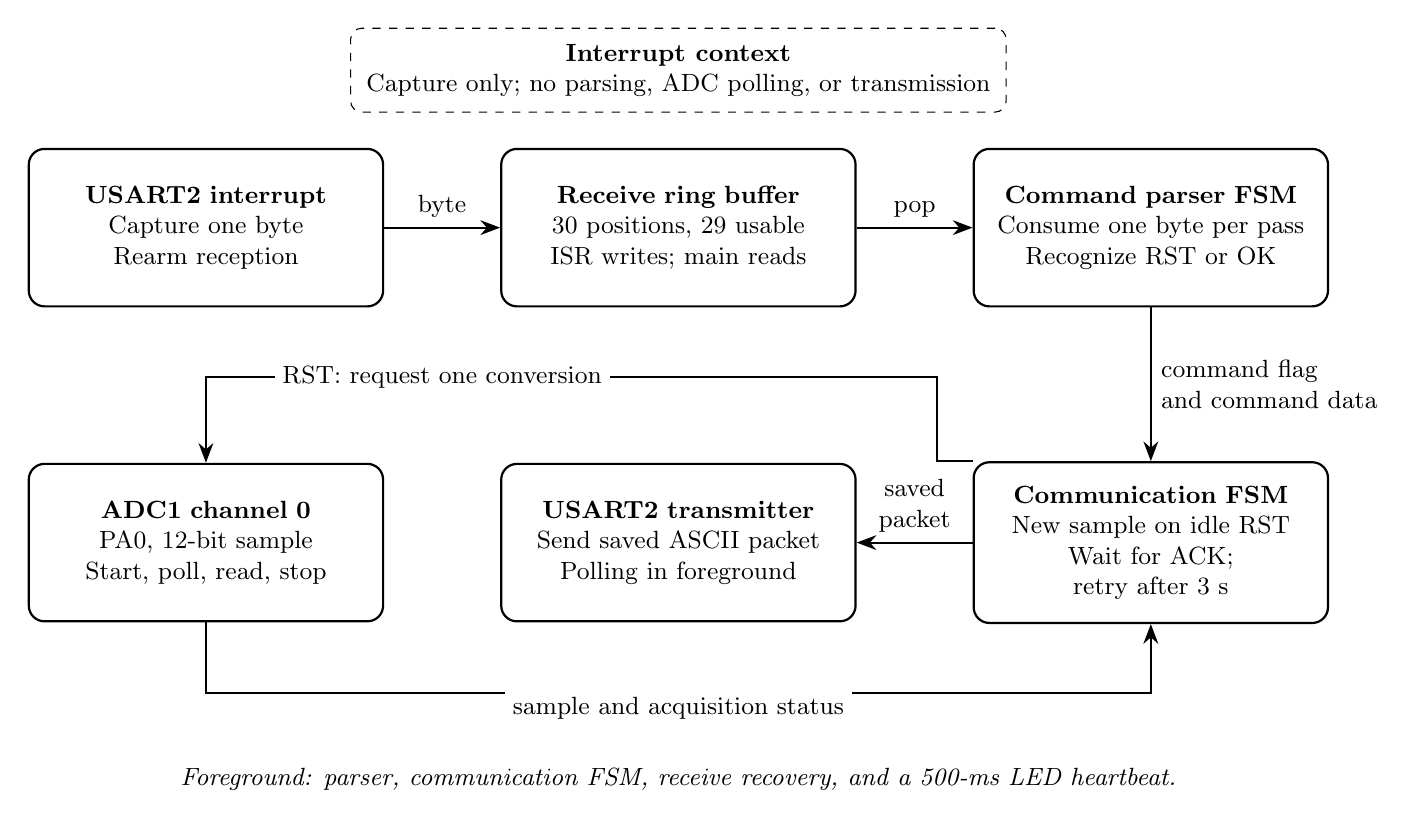
\begin{tikzpicture}[
 font=\small,
 state/.style={circle,draw,thick,minimum size=30mm,align=center,inner sep=1mm,font=\small\bfseries},
 labelbox/.style={align=center,font=\small,inner sep=2mm,fill=white},
 flow/.style={-{Stealth[length=2.5mm]},thick},
 block/.style={draw,rounded corners=2mm,thick,align=center,text width=39mm,minimum height=20mm,inner sep=3mm}]

\node[block] (irq) at (0,0) {\textbf{USART2 interrupt}\\Capture one byte\\Rearm reception};
\node[block] (queue) at (6,0) {\textbf{Receive ring buffer}\\30 positions, 29 usable\\ISR writes; main reads};
\node[block] (parser) at (12,0) {\textbf{Command parser FSM}\\Consume one byte per pass\\Recognize RST or OK};
\node[block] (adc) at (0,-4) {\textbf{ADC1 channel 0}\\PA0, 12-bit sample\\Start, poll, read, stop};
\node[block] (tx) at (6,-4) {\textbf{USART2 transmitter}\\Send saved ASCII packet\\Polling in foreground};
\node[block] (comm) at (12,-4) {\textbf{Communication FSM}\\New sample on idle RST\\Wait for ACK; retry after 3 s};
\draw[flow] (irq) -- node[above,font=\small]{byte} (queue);
\draw[flow] (queue) -- node[above,font=\small]{pop} (parser);
\draw[flow] (parser) -- node[right,align=left]{command flag\\and command data} (comm);
\draw[flow] (comm) -- node[above,font=\small,align=center]{saved\\packet} (tx);
\draw[flow] (comm.north west) -- ++(-.45,0) |- (0,-1.9) -- (adc.north);
\node[fill=white,font=\small,inner sep=1mm] at (3,-1.9) {RST: request one conversion};
\draw[flow] (adc.south) -- ++(0,-.9) -| (comm.south);
\node[fill=white,font=\small,inner sep=1mm] at (6,-6.1) {sample and acquisition status};
\node[draw,dashed,rounded corners,inner sep=2mm,align=center] at (6,2) {\textbf{Interrupt context}\\Capture only; no parsing, ADC polling, or transmission};
\node[align=center,font=\small\itshape] at (6,-7) {Foreground: parser, communication FSM, receive recovery, and a 500-ms LED heartbeat.};

\end{tikzpicture}
\end{document}
